\documentclass{article}
\usepackage[top=1in,bottom=1in,left=1in,right=1in]{geometry}
\usepackage[utf8]{inputenc}
\usepackage{graphicx}
\usepackage{xcolor}
\usepackage{amsmath}
\usepackage{systeme,mathtools}
\usepackage{pgfplots}
\pgfplotsset{compat=1.16}
\usepackage{empheq,etoolbox}


\title{Linear Algebra (MIT 18.06 Spring 2005) Notes}
\author{Simon Ebel}
\date{August 2022}

\begin{document}

\maketitle

\section{The Geometry of Linear Equations}
We consider the case where we have n linear equations with n unknowns.
This linear equations can be seen from three differents views
\begin{itemize}
    \item Row Picture
    \item Column Picture
    \item Matrix Form
\end{itemize}
Now lets consider the following example in two dimensions :
\begin{subequations}
    \begin{empheq}[left=\empheqlbrace]{align}
        2x-y=0 \\
        -x+2y=3
    \end{empheq}
\end{subequations}
Which can be put in the matrix form:
\begin{equation}
    AX=b
\end{equation}
\begin{gather}
    \begin{bmatrix} 2 & 1 \\ -1 & 2 \end{bmatrix}
    \begin{bmatrix}
        x \\
        y
    \end{bmatrix}
    =
    \begin{bmatrix}
        0 \\
        3
    \end{bmatrix}
\end{gather}
The idea is to solve this example and step back to see the biggest picture of Linear Algebra

\subsection{Row Picture}
We take one row at a time and we plot the points that satisfy the rows. Is't often good to start we the horizontal line.
\hspace{3cm}
\begin{center}
    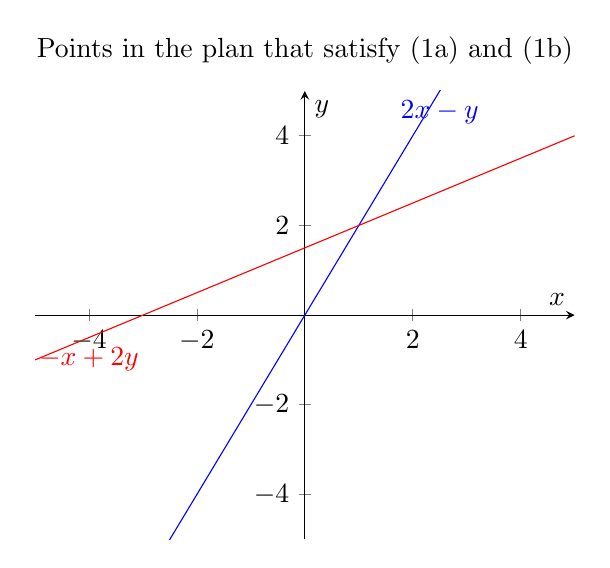
\begin{tikzpicture}% coordinates%\begin{}[]%\addplot coordinates {};%\end{}%\end{}
        \begin{axis}[
                title={Points in the plan that satisfy (1a) and (1b)},
                axis x line=middle,
                axis y line=middle,
                ylabel=$y$,
                xlabel=$x$,
                xmin=-5,
                ymin=-5,
                xmax=5,
                ymax=5,]
            \addplot[samples=2, color=blue]{2*x}
            node[pos=0.75,below] {$2x-y$};
            \addplot[samples=2, color=red]{(3+x)/2}
            node[pos=0.1,below] {$-x+2y$};

        \end{axis}

    \end{tikzpicture}
\end{center}

\end{document}
